\epigraph{\textit{Information flow is what the Internet is about. Information sharing is power. If you don't share your ideas, smart people can't do anything about them, and you'll remain anonymous and powerless.}}{-- \textup{Vint Cerf}}

We have seen thus far the two main export formats supported by Wikidata, namely, RDF and JSON. However, none of them are suitable for analytical queries. In this chapter, we will explore the possibility of exporting Wikidata in a columnar format, as we have mentioned in the previous chapter, DuckDB is the perfect candidate for this task. Putting this all together, we will create a Rust-based solution for exporting Wikidata to DuckDB.

\section{The issue with JSON and other text-based formats}

JSON is a text-based format, and as such, the data that is stored inside a JSON file is not compressed in any way. This means that the size of the file is directly proportional to the size of the data. This is not a problem for small datasets, but it becomes an issue when we are dealing with larger information repositories. As we have seen in the introductory chapter a Wikidata JSON dump is around \texttt{1.5 TB} in size when uncompressed, see \ref{chapter:intro} for a more detailed explanation. The problem here is that we cannot store such a large file on a single machine. Even if we could, it would take quite a time to load the whole file into memory. As a result, a binary format is required to store the information. This is where DuckDB comes into play. Even if we are also required to load the database into memory; recall, DuckDB is an in-process or embedded database, and the size of the repository is much smaller than the one of the JSON file; orders of magnitude smaller to say the least. This is because DuckDB is a columnar database, and as such, it can compress the data much more efficiently than a text-based format. This is the main reason why we want to export Wikidata to DuckDB.

It is also worth noting that Wikidata JSON dumps are structured in such a way that per each line of the file, one object is stored. This means that we can parse the file line by line, which is something cool. However, it comes with the downside that every line of the dump will contain boilerplate information referring to the schema of the JSON objects. What I mean by this, is that we will potentially have hundreds of millions of lines all of them with the same boilerplate code. Instead of having a header with the schema of the JSON object, we will have it in every line. This is one of the reasons why JSON files are not efficient memory-wise. For sharing information, JSON is great, but for storing it, it is not.

\section{wd2duckdb}

Now that we have a clear understanding of the scope of the project, we can start working on the design of the tool in charge of transforming the Wikidata JSON dumps into a DuckDB file. For us to do so, some restrictions are going to be considered. First, we are interested in storing only one of the translations for each Wikidata entity; that is, we are going to store only one of the labels, descriptions, and aliases for each item. The language of choice can be modified\footnote{\url{https://github.com/angelip2303/wd2duckdb/blob/master/wikidata-rs/src/lib.rs\#L20}}. Second, we are going to store only the statements that are not deprecated. Apart from that, the rest of the information is going to be preserved.

\label{section:wd2duckdb_design}
\subsection{Design}

The tool is going to be divided into two main parts. The first part is going to be in charge of parsing the Wikidata JSON dump and extracting the information that we are interested in. The second part is going to be in charge of storing the information in a DuckDB database. The idea is to allow backends to be interchangeable; that is, several implementations for other drivers should be implemented without actually changing the existing code. However, for the sake of simplicity, we are going to focus on DuckDB for the time being.

\begin{figure}[ht]
    \centering
    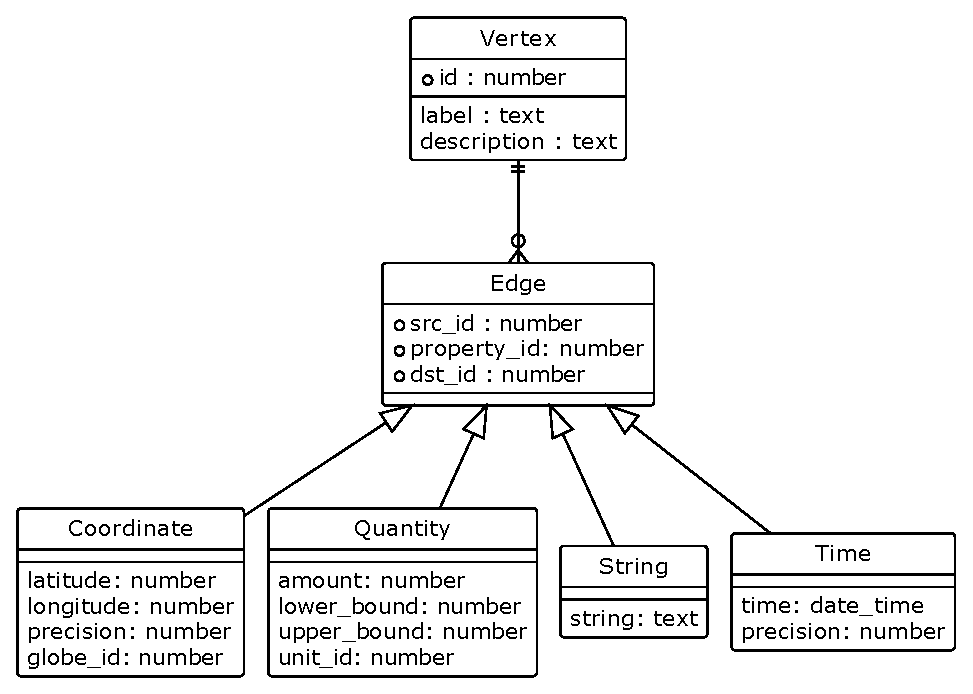
\includegraphics[width=.8\linewidth]{img/10-1_wd2duckdb.eps}
    \caption{Entity-relationship diagram of \texttt{wd2duckdb}'s resulting Database}
\end{figure}%